\begin{frame}{Zaprojektowane komoponenty systemu testowego}

%     \begin{figure}[H]
%         \centering
%         \begin{subfigure}[b]{0.65\textwidth}
%             \centering
%             \includegraphics[width=\textwidth]{ch5/IMG_3725.jpg}

%         \end{subfigure}
%         \hfill
%         \begin{subfigure}[b]{0.3\textwidth}
%             \centering
%             \includegraphics[width=\textwidth]{ch5/chip.jpg} 
%             \includegraphics[width=\textwidth]{ch5/asic_photo.jpg}
%         \end{subfigure}     

%    \end{figure}
\begin{columns}
    \column{.57\textwidth}
    \vspace{-1em}

    \begin{figure}[H]
    \centering
        \includegraphics[width=\textwidth]{ch5/IMG_3725.jpg}
    \end{figure}

    \column{.4\textwidth}
\vspace{-1em}
    \begin{figure}[H]
    \centering
        \includegraphics[width=\textwidth]{ch5/inputfile_A0.01VPP_vibias0.0_ictrl290_corr100_0_ver02_101_par0_test_generator.png} 
        \includegraphics[width=0.9\textwidth]{ch5/asic_photo.jpg}

    \end{figure}
\end{columns}


\end{frame}


\begin{frame}{Regulacja częstotliwości granicznej}

    \begin{figure}[H]
        \centering
        \begin{subfigure}[b]{0.485\textwidth}
            \centering
            \includegraphics[scale=0.8]{scripts/tmp/bodePlotFc_2.pdf}  

        \end{subfigure}
        % \hfill
        \begin{subfigure}[b]{0.485\textwidth}
            \centering
            \includegraphics[scale=0.8]{scripts/tmp/bodePlotFc_ictrl.pdf}

        \end{subfigure}     

    \end{figure}
    \vspace{-1em}
    \begin{block}{}
        \begin{itemize}
            \item częstotliwość graniczna regulowana w zakresie od $\SIrange{0.1}{20}{\hertz}$ 
            \item jednorodność kanałów 
        \end{itemize}
    \end{block}


\end{frame}

%  

% \begin{frame}{Pomiary zniekształceń harmonicznych -- wpływ korekty}

%     \begin{columns}

%         \column{.45\textwidth}
%         \begin{block}{Brak globalnej korekty}
%             \begin{figure}[H]
%                 \centering
%                 \includegraphics[scale = 0.85]{scripts/tmp/thdFreqCorr0_0.pdf} 
%             \end{figure}   
%         \end{block}

%         \column{.45\textwidth}

%         \begin{block}{Korekta globalna}
%             \begin{figure}[H]
%                 \centering
%                 \includegraphics[scale = 0.85]{scripts/tmp/thdFreqCorr100_0.pdf}
%             \end{figure}   
%         \end{block}
%     \end{columns}

% \end{frame}

\begin{frame}{Pomiary zniekształceń}


    \begin{columns}

        \column{.45\textwidth}
\vspace{-1em}
        \begin{block}{}
            \begin{itemize}
                \item porównywalny protokół pomiarowy do symulacji -- amplituda sygnału sinusoidalnego: $\SI{10}{\milli\volt_{pp}}$
                \item zmierzony poziom zniekształceń niższy niż w symulacjach
            \end{itemize}
        \end{block}
        \vspace{-1em}

            \begin{figure}[H]
                \centering
                \includegraphics[trim={0 0.25cm 0 0.25cm}, clip, scale = 0.75]{scripts/embc2021THD_size/embc2021THD_size_0_100.pdf}
            \end{figure}   


        \column{.45\textwidth}
        \begin{figure}[H]
            \centering
            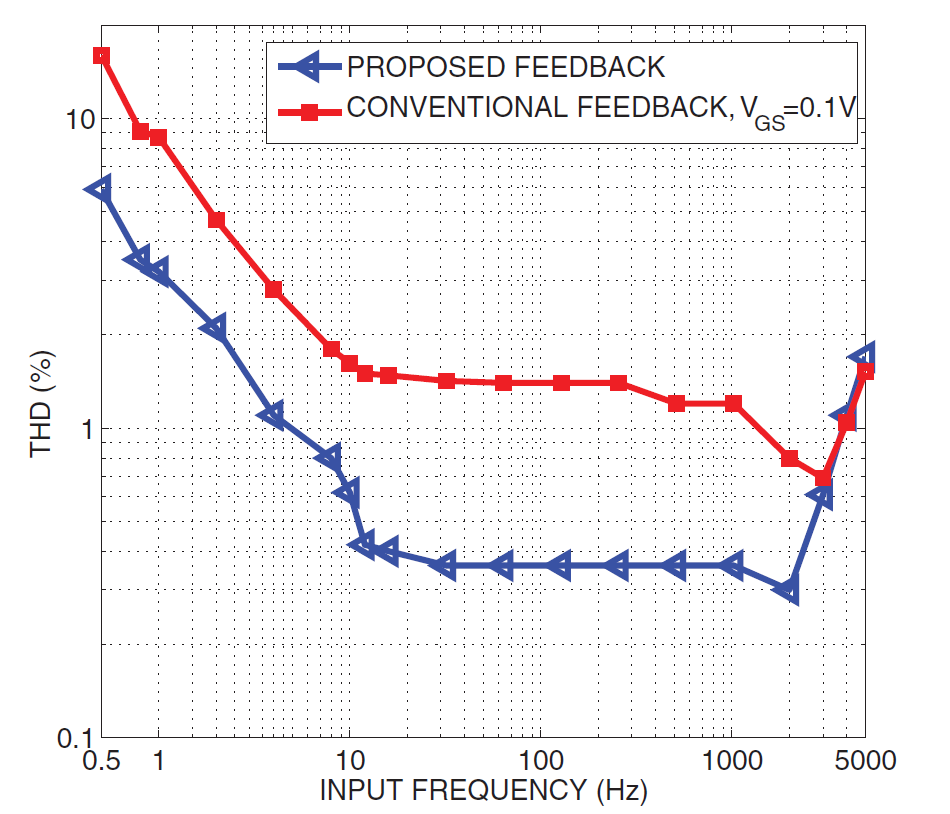
\includegraphics[scale=0.2]{Figures/genovTHD.png}
            \caption{Symulacje THD dla sygnału sinusoidalnego o amplitudzie: $\SI{1.4}{\milli\volt_{pp}}$. Na podstawie K. Abdelhalim and R. Genov, doi: 10.1109/ISCAS.2012.6271415}
        \end{figure}
\end{columns}

\end{frame}
        % \begin{block}{Drugi wariant przedwzmacniacza z większymi pojemnościami wejściowymi}


        %     \begin{figure}[H]
        %         \centering
        %         \includegraphics[trim={0 0.25cm 0 0.25cm}, clip, scale = 0.8]{scripts/embc2021THD_size/embc2021THD_size_1_100.pdf}
        %     \end{figure}   
        % \end{block}
  

    % \begin{figure}[H]
    %     \centering
    %     \begin{subfigure}{0.485\textwidth}
    %         \centering
    %         \includegraphics[trim={0 0.25cm 0 0.25cm}, clip, scale = 0.6]{scripts/embc2021THD_size/embc2021THD_size_0_0.pdf}
    %     \end{subfigure}
    %     % \hfill
    %     \begin{subfigure}{0.485\textwidth}
    %         \centering
    %         \includegraphics[trim={0 0.25cm 0 0.25cm}, clip, scale = 0.6]{scripts/embc2021THD_size/embc2021THD_size_1_0.pdf}
    %     \end{subfigure} 
    %     % \vfill
    %     \begin{subfigure}{0.485\textwidth}
    %         \centering
    %         \includegraphics[trim={0 0.25cm 0 0.25cm}, clip, scale = 0.6]{scripts/embc2021THD_size/embc2021THD_size_0_100.pdf}
    %     \end{subfigure}
    %     % \hfill
    %     \begin{subfigure}{0.485\textwidth}
    %         \centering
    %         \includegraphics[trim={0 0.25cm 0 0.25cm}, clip, scale = 0.6]{scripts/embc2021THD_size/embc2021THD_size_1_100.pdf}
    %     \end{subfigure}   
    % \end{figure}


% \begin{frame}{Pomiary szumów}
%     % \begin{figure}[H]
%     %     \centering 
%     %     \includegraphics[scale=0.4]{scripts/tmp/measurementNoiseDataset.pdf}  
%     % \end{figure}

%     \begin{figure}[H]
%         \centering
%         \begin{subfigure}[b]{0.485\textwidth}
%             \centering
%             \includegraphics{scripts/tmp/noiseGND_in.pdf}
%         \end{subfigure}
%         % \hfill
%         \begin{subfigure}[b]{0.485\textwidth}
%             \centering
%             \includegraphics{scripts/tmp/noiseElektrodaNaCl.pdf}
%         \end{subfigure}     
%     \end{figure}
% \end{frame}



\begin{frame}{Schemat eksperymentu z wykorzystaniem systemu pomiarowego}
    \begin{columns}

        \column{.5\textwidth}


        \begin{figure}[H]
            \centering 
            \includegraphics[scale=0.175]{ch6/setupIBDtot.png}  
        \end{figure}

        \column{.45\textwidth}
        \vspace{-1em}

        \begin{block}{}

            \begin{itemize}
                \item Sonda komercyjna firmy Neuronexus -- 16 elektrod na trzpieniu sondy
                \item Wymuszona aktywnosć: Sonda w obszarze kory mózgowej na głębokości $\SI{1.4}{\milli\metre}$ pod powierzchnią mózgu
                \item Spontaniczna aktywnosć: Sonda w obszarze wzgórza a głębokości $\SI{6}{\milli\metre}$ pod powierzchnią mózgu


            \end{itemize}
            \vspace{-1em}

            \begin{figure}[H]
                \centering 
                \includegraphics[scale=0.1]{ch6/tissueDescription.png}  
            \end{figure}
        \end{block}



    \end{columns}

\end{frame}

% \begin{frame}{}
%     \begin{figure}[H]
%        % \begin{subfigure}{0.3\textwidth}
   
%        %  \end{subfigure}
%        %      \hfill
   
%        \begin{subfigure}{0.25\textwidth}
%            \includegraphics[scale = 0.75]{ch6/meaLFPnexus.pdf}
%             % \vfill
%         \end{subfigure}
%        % \hfill
%            \hspace{-5em}
%         \begin{subfigure}{0.7\textwidth}
%            \includegraphics[scale = 0.75]{scripts/tmp/signal_MEA_LFP_wide.pdf}
%         \end{subfigure}
%    \end{figure}
% \end{frame}

\begin{frame}{Aktywność neuronalna zarejestrowana przez HiFiNeuroPre}
    \begin{columns}

        \column{.6\textwidth}
        \vspace{-1em}

        \begin{block}{}
            {\renewcommand\normalsize{\small}%
            \normalsize
            \begin{itemize}
                \item Stymulacja zewnętrzna  aplikowana cyklicznie w różnych odstępach czasu -- od $\SIrange{3}{5}{\second}$;
                \item 60 powtórzeń stymulacji w danym cyklu pomiarowym 
                \item Kilka cykli pomiarowych dla różnych ustawień sprzętu
    
            \end{itemize}
            }
            \vspace{-1em}
        \begin{figure}[H]
            % \begin{subfigure}{0.3\textwidth}
        
            %  \end{subfigure}
            %      \hfill
        
            \begin{subfigure}{0.25\textwidth}
                \includegraphics[scale = 0.45]{ch6/meaLFPnexus.pdf}
                 % \vfill
             \end{subfigure}
            % \hfill
                \hspace{-2em}
             \begin{subfigure}{0.7\textwidth}
                \includegraphics[scale = 0.45]{scripts/tmp/signal_MEA_LFP_wide.pdf}
             \end{subfigure}
        \end{figure}
        \end{block}
        \column{.35\textwidth}
        \vspace{-1em}

        \begin{block}{Zapis spontanicznej aktywności neuronalnej}
            \begin{figure}[H]
                \centering
                \includegraphics[scale=0.6]{scripts/tmp/signal_MEA_AP_2.pdf}
        \end{figure}
        \end{block}

    \end{columns}
        

    % \begin{figure}[H]
    %     \centering
    %     \begin{subfigure}[b]{0.485\textwidth}
    %         \centering
    %         \includegraphics[scale=0.8]{scripts/tmp/signal_MEA_AP_1.pdf}
    %         \caption{}
    %     \end{subfigure}
    %     % \hfill
    %     \begin{subfigure}[b]{0.485\textwidth}
    %         \centering
    %         \includegraphics[scale=0.8]{scripts/tmp/signal_MEA_AP_2.pdf}
    %         \caption{}
    %     \end{subfigure}     
    % \end{figure}
\end{frame}

